\documentclass[class=report, crop=false, 12pt,a4paper]{standalone}
\usepackage{enumitem}
\usepackage{float}
\usepackage[normalem]{ulem}
\usepackage{graphicx}
\usepackage{amsmath}
\usepackage{siunitx}
\usepackage{commath}
\usepackage{tikz}
\usetikzlibrary{positioning, fit, calc}   
\tikzset{block/.style={draw, thick, text width=3cm ,minimum height=1.3cm, align=center},   
line/.style={-latex}     
}  
\begin{document}
\section{Differential analysis of fluid flow}
What do we want to know? The velocity field, pressures, densities and temperature everywhere and anytime. Hence, these will be a function of (x, y, z, t).

List of variables
\begin{center}
  \begin{tabular}{||c c c||} 
  \hline
  Variable & Type & Units \\ [0.5ex] 
  \hline\hline
  $\begin{matrix}
    \overrightarrow{U} = u \hat{i} + v\hat{j} + w\hat{k}\\
    \overrightarrow{U} = u_1 \hat{i}_1 + u_2 \hat{i}_2 + u_3 \hat{i}_3
  \end{matrix}$ & Velocity/Vector & \si{\m\per\s}\\ 
  \hline
  $p$ & Pressure/Scalar & \si{\newton\per\meter\squared} \\
  \hline
  $T$ & Temperature/Scalar & \si{\celsius} \\
  \hline
  $\rho$ & Density/Scalar & \si{\kg\per\meter\cubed} \\
  \hline
  $T = \begin{bmatrix}
    \tau_{xx} & \tau_{xy} & \tau_{xz}\\
    \tau_{yx} & \tau_{yy} & \tau_{yz}\\
    \tau_{zx} & \tau_{zy} & \tau_{zz}
  \end{bmatrix}$ & Stress Tensor & \si{\newton\per\meter\squared} \\ [1ex] 
  \hline
 \end{tabular}
\end{center}
Since we have 12 variables, we need 12 equations to describe the fluid!

From last year, we have our conservation of mass equation
$$\frac{\partial}{\partial t} \int_V \rho \dif V + \oint_S (\rho \overrightarrow{V} \cdot \hat{n} )\dif S = 0$$
\begin{figure}
  \centering
  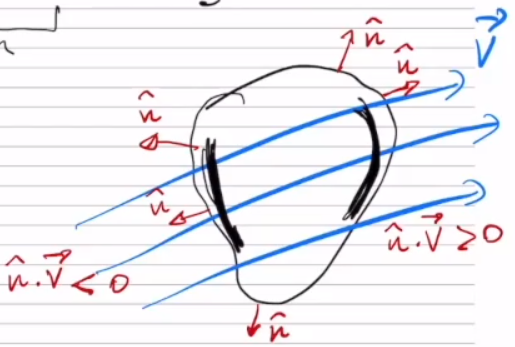
\includegraphics[width = 0.8\textwidth]{../img/euleriancontrolvolume.png}
  \caption{Consider $\hat{n}$ to be a vector coming out of the control volume. Depending on where $\hat{n}$ is, our dot product will either be greater than or less than 0.}
\end{figure}
\begin{figure}
  \centering
  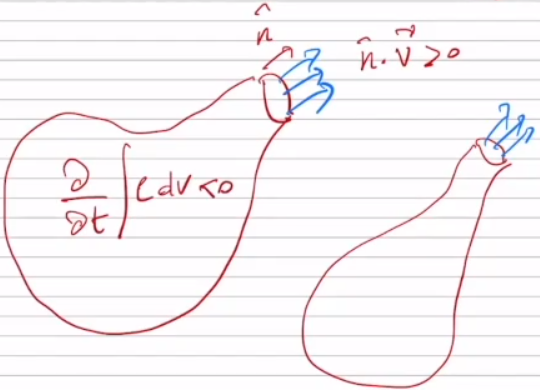
\includegraphics[width = 0.8 \textwidth]{../img/balloondeflatingeg.png}
  \caption{There is a velocity exiting the balloon. The amount of mass inside will decrease with time. The volume of the balloon will become smaller. This will be equal to the amount of mass which came out of the control volume (the balloon). If the second term of the continuity equation is postive, the first term must be negative.}
\end{figure}
\end{document}